
\section{needle}

\begin{frame}[c]{needle - Introduction}
    \begin{itemize}
    \item Sequence based Algorithm \newline
    \pause
    \item part of the EMBOSS package \newline
    \pause
    \item Implementation of the Needleman-Wunsch algorithm
    \end{itemize}
\end{frame}


\begin{frame}[c]{Needleman-Wunsch Algorithm}
    Sometimes also called: \newline
    \begin{itemize}
    \pause
    \item Optimal matching algorithm \newline
    \pause
    \item Global alignment technique
    \end{itemize}
\end{frame}


\section{Sequence Alignment}

\begin{frame}[c]{Sequence Alignment}
    \begin{itemize}
    \item local sequence alignment \newline
    \pause
    \item global sequence alignment \newline
    \pause
    \item glocal sequence alignment
    \end{itemize}
\end{frame}


\begin{frame}[c]{Sequence Alignment - local}
    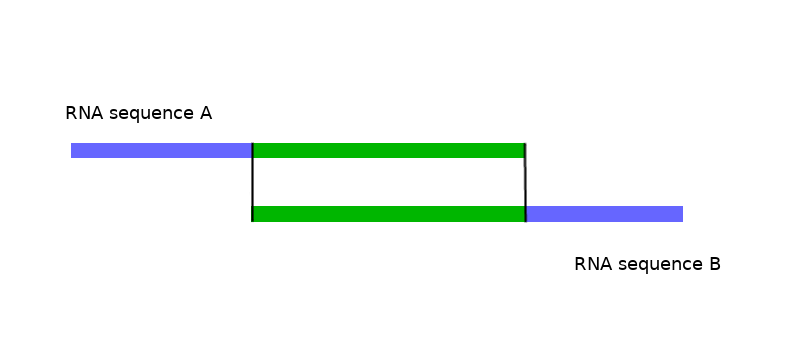
\includegraphics[width=\textwidth]{rna_comparison_local}
\end{frame}

\begin{frame}[c]{Sequence Alignment - global}
    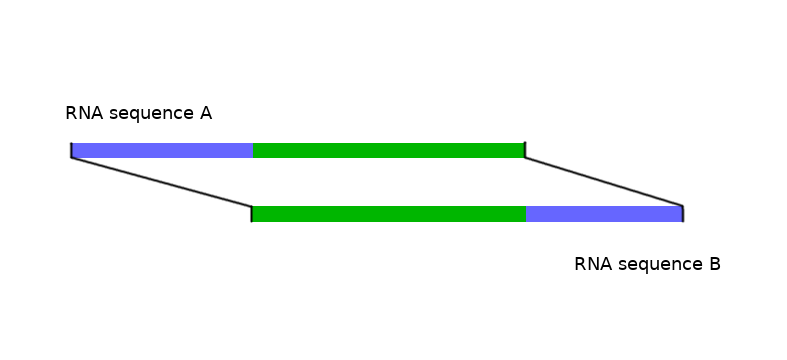
\includegraphics[width=\textwidth]{rna_comparison_global}
\end{frame}

\begin{frame}[c]{Sequence Alignment - glocal}
    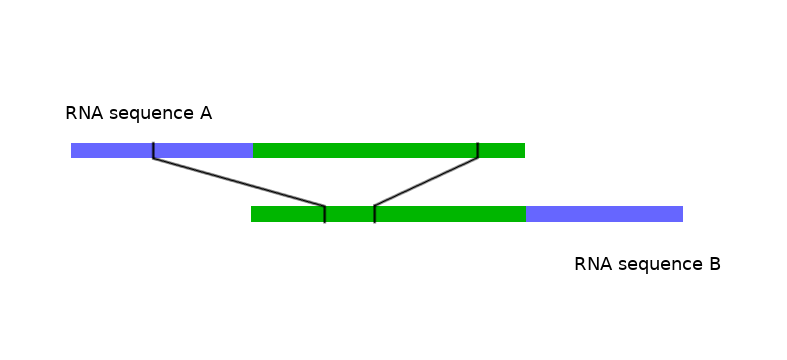
\includegraphics[width=\textwidth]{rna_comparison_glocal2}
\end{frame}


\section{Needleman-Wunsch}


\begin{frame}[c]{Needleman-Wunsch Algorithm - introduction}

    We need a scoring system. \newline \newline
    \pause
    Example: \pause
    \begin{itemize}
    \item Match: 1
    \item Mismatch: -1
    \item Indel: -1
    \end{itemize}

\end{frame}


\begin{frame}[c]{Needleman-Wunsch Algorithm}
    Two sequences to compare: \newline \newline
    \pause
    GCATGCU \newline
    GATTACA
\end{frame}

% tables in latex: https://en.wikibooks.org/wiki/LaTeX/Tables
\begin{frame}[c]{Needleman-Wunsch Algorithm - Example}
    \center
    \begin{tabular}{|c|c|c|c|c|c|c|c|c|}
    \hline
    \phantom{A} & \phantom{A} & \bf{G} & \bf{C} & \bf{A} & \bf{T} & \bf{G} & \bf{C} & \bf{U} \\
    \hline
    \phantom{A} & \onslide<2->{0} & \onslide<3->{-1} & \onslide<3->{-2} & \onslide<3->{-3} & \onslide<3->{-4} & \onslide<3->{-5} & \onslide<3->{-6} & \onslide<3->{-7} \\ \hline
    \bf{G} & \onslide<3->{-1} & \only<4-4>{X} \only<5->{1} & \only<6-6>{X} \only<7->{0} & \only<8->{-1} & \only<8->{-2} & \only<8->{-3} & \only<8->{-4} & \only<8->{-5} \\ \hline
    \bf{A} & \onslide<3->{-2} & \only<6-6>{Y} \only<7->{0} & \only<8->{0} & \only<8->{1} & \only<8->{0} & \only<8->{-1} & \only<8->{-2} & \only<8->{-3} \\ \hline
    \bf{T} & \onslide<3->{-3} & \only<8->{-1} & \only<8->{-1} & \only<8->{0} & \only<8->{2} & \only<8->{1} & \only<8->{0} & \only<8->{-1} \\ \hline
    \bf{T} & \onslide<3->{-4} & \only<8->{-2} & \only<8->{-2} & \only<8->{-1} & \only<8->{1} & \only<8->{1} & \only<8->{0} & \only<8->{-1} \\ \hline
    \bf{A} & \onslide<3->{-5} & \only<8->{-3} & \only<8->{-3} & \only<8->{-1} & \only<8->{0} & \only<8->{0} & \only<8->{0} & \only<8->{-1} \\ \hline
    \bf{C} & \onslide<3->{-6} & \only<8->{-4} & \only<8->{-2} & \only<8->{-2} & \only<8->{-1} & \only<8->{-1} & \only<8->{1} & \only<8->{0} \\ \hline
    \bf{A} & \onslide<3->{-7} & \only<8->{-5} & \only<8->{-3} & \only<8->{-1} & \only<8->{-2} & \only<8->{-2} & \only<8->{0} & \only<8->{0} \\ \hline

    \end{tabular}
\end{frame}


\begin{frame}[c]{Needleman-Wunsch Algorithm - Best Matches}
    \center
%     % trim = l b r t
%     \includegraphics[width=\textwidth, clip=true, trim = 300mm 370mm 300mm 370mm]{cogbias}
    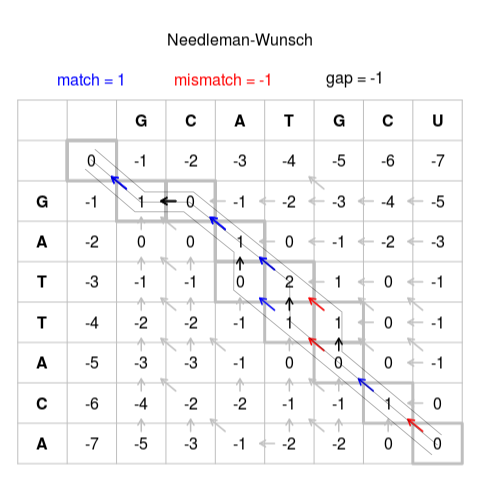
\includegraphics[width=.8\textwidth, clip=true, trim = 0mm 0mm 0mm 25mm]{Needleman-Wunsch_pairwise_sequence_alignment}
\end{frame}


\begin{frame}[c]{Needleman-Wunsch Algorithm - Results}
    \begin{tabular}{l|lll}
    Sequences & \multicolumn{3}{ c }{Best alignments} \\
    \hline
    GCATGCU      & GCATG-CU      & GCA-TGCU      & GCAT-GCU \\
    GATTACA      & G-ATTACA      & G-ATTACA      & G-ATTACA
    \end{tabular}
\end{frame}


